\documentclass[12pt,letterpaper]{article}
\usepackage[top=1.5 in, bottom = 1.5 in, left = 1 in, right=1 in]{geometry}
\usepackage[american]{babel}
\usepackage[numbers]{natbib}
\usepackage{tocloft}
\usepackage{bookmark}
\usepackage{etoolbox}
\apptocmd{\thebibliography}{\raggedright}{}{}
\usepackage{amsmath}
\usepackage{amssymb, amsfonts, textcomp}
\usepackage{titlesec}
\usepackage{color}
\usepackage{multicol}
\usepackage{multirow}
\usepackage{tabu}
\usepackage{booktabs}
\usepackage{array}
\usepackage{hhline}
\usepackage{hyperref}
\usepackage{framed}
\usepackage{fontspec}
\setmainfont{Chaparral Pro}
\setromanfont{Chaparral Pro}
\setmonofont{Consolas}
\setsansfont{Myriad Pro}
\setcounter{secnumdepth}{5}
\pagestyle{plain}

%\titleformat{<command>}[<shape>]{<format>}{<label>}{<sep>}{<before-code>}[<after-code>]
\titleformat{\subparagraph}[hang]
{\normalfont\normalsize\bfseries}{\thesubparagraph}{1 em}{}[]
%\titlespacing*{<command>}{<left>}{<before-sep>}{<after-sep>}
\titlespacing*{\subparagraph}{0 pt}{2 ex}{.25 ex}

\titleformat{\paragraph}[hang]
{\normalfont\normalsize\bfseries}{\theparagraph}{1 em}{}[]
\titlespacing*{\paragraph}{0 pt}{2 ex}{.25 ex}

\begin{document}
	\pagenumbering{gobble}
	\vspace*{2.8 in}
	\begin{huge}
		\begin{center}
			User Documentation
			\par
			for
			\par
			The Walking Game
			\par
		\end{center}
	\end{huge}
	\vspace*{2.5 in}
	\begin{large}
		\begin{flushright}
			Star Team
			
			Version: 1.0
			
			Date: 11/14/2014
		\end{flushright}
	\end{large}
	
	\clearpage
	\section*{Revision History}
	\begin{flushleft}
		\begin{tabular}{|p{0.14\linewidth}|p{0.12\linewidth}|p{0.45\linewidth}|p{0.18\linewidth}|}
			\hline
			\textbf{Revision \#} & \textbf{Date} & \textbf{Description} & \textbf{Author} \\\hline
			1.0 & 10/31/2014 & Initial revision & Samuel I. Gunadi \\\hline
		\end{tabular}
	\end{flushleft}
	\clearpage
	
	\clearpage
	\tableofcontents
	
	\clearpage
	\setcounter{page}{0}
	
	\pagenumbering{arabic}
	
	\section{Definitions, acronyms, and abbreviations}
	OpenGL --- Open Graphics Library
	
	\vspace{0.1in}\noindent OBJ --- Wavefront OBJ File Format
	
	\vspace{0.1in}\noindent GLEW --- The OpenGL Extension Wrangler Library 
	
	\vspace{0.1in}\noindent PDF --- Portable Document Format
	
	\vspace{0.1in}\noindent IDE --- Integrated Development Environment
	
	\vspace{0.1in}\noindent MMORPG --- Massively Multiplayer Online Role-Playing Game
	
	\section{Introduction}
	The members of Star team are Samuel I. Gunadi, Roberto J. Kondurura, and Ryan Elegant. The project website can be found at \begin{footnotesize}\url{https://github.com/samuelgunadi/thewalkinggame}\end{footnotesize}.
	
	The Walking Game features a Wavefront OBJ file parser; people 3D models, textures, and walking animations; textures with alpha blending; a textured floor; collision detection; simple command interpreter and scripting; nameplates; and an MMORPG style third-person camera. 
	
	The animation technique used in The Walking Games will not be skeletal animation; instead, it will be by loading one .obj for every key frame. This results in very large files.
	\section{User interfaces}
	The Walking Game includes an interface resembling an RPG game with a console to provide additional functionalities and aid in testing and debugging process.
	
	\section{Hardware requirements}
	The Walking Game should run on any computer hardware meeting the following criteria:
	\begin{itemize}
	\item Dual-core CPU
	\item OpenGL 4.3 compatible GPU with 2 GB memory
	\item 2 GB free hard disk space.
	\item Mouse with 3 buttons
	\item Keyboard with US layout
	\item 2 GB of RAM
	\end{itemize}
	
	\section{Character control}
	
	\begin{tabular}{| l | l |} \hline
	\textbf{Input} & \textbf{Action} \\\hline
	Esc & Exit the program \\\hline
	W, S & Move forward/backward \\\hline
	A, D & Turn left/right\\\hline
	Left, right & Pan camera\\\hline
	Up, down & Tilt camera\\\hline
	Page down, page up & Dolly camera\\\hline
	Mouse wheel & Dolly camera\\\hline
	Left click and drag & Pan and tilt camera\\\hline
	Right click and drag & Pan and tilt camera and turn\\\hline
	\end{tabular}
	
	\section{Console commands}
	
	Available commands:
	
	\begin{framed}
		\footnotesize
		\begin{verbatim}
		help
		exit
		showallnames
		createnpc [string:name] [int:model_id]
		createnpc [string:name] [int:model_id] [float:x] [float:y] [float:z]
		deletenpc [string:name]
		setmodel [string:name] [int:model_id]
		getmodelinfo [string:name]
		setwalkingspeed [string:name] [float:speed]
		getwalkingspeed [string:name]
		setposition [string:name] [float:x] [float:y] [float:z]
		getposition [string:name]
		setangle [string:name] [float:angle]
		getangle [string:name]
		setanimationstate [string:name] [int:state]
		getanimationstate [string:name]
		takecontrol [string:name]
		getcamerainfo
		setcamerapos [float:x] [float:y] [float:z]
		setcameratarget [float:x] [float:y] [float:z]
		setcameraradius [float:radius]
		getlightinfo
		setlightpos [float:x] [float:y] [float:z]
		setlightintensity [float:r] [float:g] [float:b]
		setfpslimit [int:fps]
		sleep [double:seconds] -- pause (for scripting)
		loadscript [string:path] -- the file must be in ASCII encoding
		    (sample script can be found in /binary/testscript.txt)
		test -- for testing purposes
		\end{verbatim}
		\normalsize
	\end{framed}
	NOTE---All strings must not contain spaces.
	
	\section{Third-party libraries}
	The Walking Game integrates several external software to provide functionality:
	\begin{enumerate}
		\item GLFW. GLFW is used for creating windows with OpenGL contexts and receiving input and events. GLFW is multi-platform and supports Windows, OS X and many Unix-like systems. GLFW is licensed under the zlib/libpng license.
		
		\item GLEW. GLEW is a cross-platform open-source C/C++ extension loading library. GLEW provides efficient run-time mechanisms for determining which OpenGL extensions are supported on the target platform. OpenGL core and extension functionality is exposed in a single header file. GLEW has been tested on a variety of operating systems, including Windows, Linux, Mac OS X, FreeBSD, Irix, and Solaris.
		
		\item GLM. GLM is a header only C++ mathematics library for graphics software based on the OpenGL Shading Language (GLSL) specification and released under the MIT license.
	\end{enumerate}
	
	\hypertarget{appendixa}{}
	\bookmark[level=section, dest=appendixa]{Appendix A: Screenshots}
	\addcontentsline{toc}{section}{Appendix A: Screenshots}
	\section*{Appendix A: Screenshots}
	\begin{figure}[h]
	\centering
	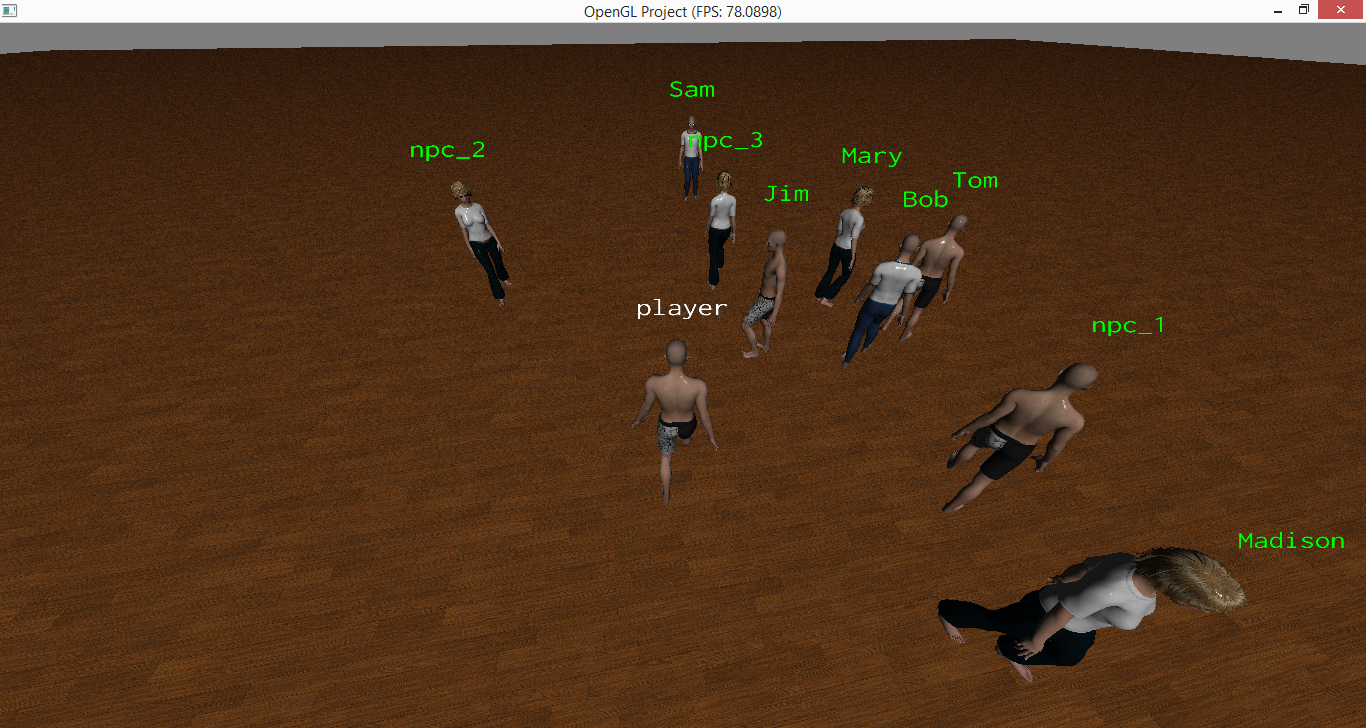
\includegraphics[width=\linewidth]{screenshot1}
	\caption{Main window of The Walking Game}
	\label{fig:screenshot1}
	\end{figure}
	\begin{figure}[h]
	\centering
	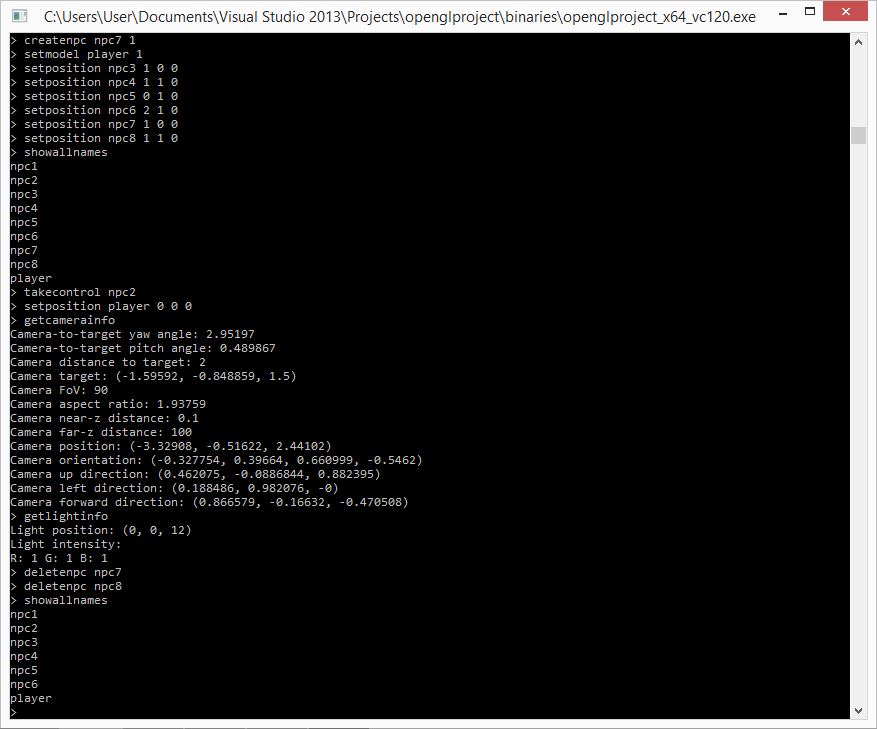
\includegraphics[width=\linewidth]{screenshot2}
	\caption{Console commands example \#1}
	\label{fig:screenshot2}
	\end{figure}
	\begin{figure}[h]
	\centering
	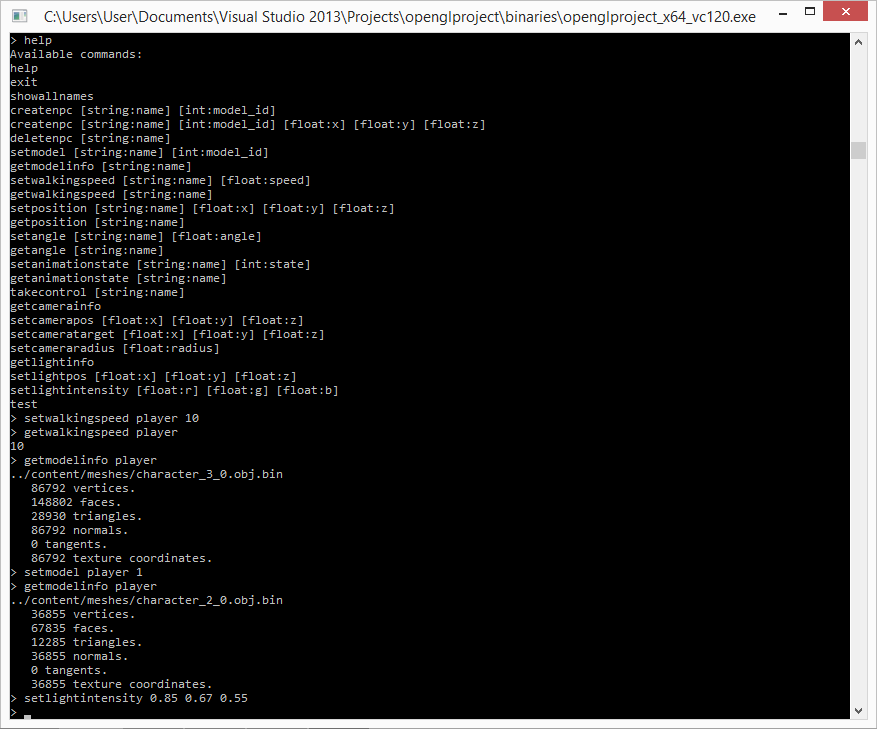
\includegraphics[width=\linewidth]{screenshot3}
	\caption{Console commands example \#2}
	\label{fig:screenshot3}
	\end{figure}
	\clearpage
	
	\nocite{*}
	
	\addcontentsline{toc}{section}{References}
	\bibliographystyle{IEEEtranN}
	\bibliography{references}

\end{document}
